% Supplementary numerical experiments.
% Required packages: amsmath, booktabs, graphicx, and xcolor.
% Figure paths are relative to this file's directory.

\begingroup
\color{blue}
\setlength{\emergencystretch}{2em}

\section{Additional Numerical Results}
\label{app:additional-experiments}

We examine how coordinate heterogeneity, dependence, calibration size, noise
tails, and residual transformations affect the coverage and efficiency of
TSCP. Comparisons with the population oracle and the unenclosed local union
separate the statistical and computational effects of its approximations.
Real-data marginal coverage and search-regime measurements complement the
results in Section~\ref{sec:numerical-experiments}.

\subsection{Experimental Protocols}
\label{app:experimental-protocols}
\label{app:legacy-experiments}

Synthetic features have ten independent standard normal coordinates, and
the outcome model is
\begin{equation}
  Y_j=f_j(\boldsymbol X)+\epsilon_j,\qquad j\in[d],
  \label{eq:data-generator}
\end{equation}
where each $f_j$ is linear with coefficients drawn from
$\operatorname{Unif}(-10,10)$ and fixed across repetitions. Noise laws and
output dimension are specified below. Ordinary least squares is used for
absolute-residual comparisons, and all methods in each repetition share
the fitted predictor. Coverage, normalized residual-space volume, full
interval lengths, and construction time follow the definitions in
Section~\ref{sec:experiment-methods}. Unless specified otherwise,
$d=10$, the target coverage is $0.9$, and results average 200 repetitions.

\paragraph{Independent-observation protocol.}
The dependence, heterogeneity, calibration-size, target-level, and
contamination sweeps independently generate 7,200 training observations,
800 test observations, and a calibration sample in each repetition.
The same protocol is used for Figure~\ref{fig:app-heavy-tails}.
The CQR experiments instead use 2,400 training and 600 test observations
over 30 repetitions; the shape-template comparison uses these sample sizes
over 100 repetitions. Calibration data are generated separately from
training and test data. Conditional on the fixed regression coefficients,
these repetitions are independent population draws.

\paragraph{Fixed-pool protocol.}
The independent-noise distribution benchmarks in
Appendix~\ref{app:simulations}, the oracle and approximation comparisons in
Appendix~\ref{app:ours_simulation}, and Figure~\ref{fig:t} use a simulated
pool of 8,000 observations for each setting. Each repetition randomly splits
this pool into 6,400 training and 1,600 test observations and generates a
separate calibration sample. The distribution benchmarks use
$n\in\{30,50,100,300,500\}$; other calibration sizes and repetition counts
are specified with their results. Variation under this protocol includes
random splitting and calibration sampling conditional on the simulated
pool, rather than variation over independently generated training/test
datasets. Results from the two protocols are not pooled.

The real-data studies use the training/calibration/test allocations and
models in Section~\ref{sec:real-data-experiments}. Coordinate-wise and
search-regime results share the evaluation batch described in
Section~\ref{sec:real-data-diagnostics}.

\FloatBarrier
\subsection{Independent-Noise Distribution Benchmarks}
\label{app:simulations}
\label{app:legacy-supplement}

The following comparisons use the fixed-pool protocol with independent
noise coordinates and calibration sizes $n\in\{30,50,100,300,500\}$.

Figure~\ref{fig:gaussian-heter} and Table~\ref{tab:gaussian-heter} examine
independent Gaussian noise with heterogeneous variance across dimensions:
\[
\epsilon^{\mathrm{heter}}_j \sim \mathcal{N}\left(0,\; (10 - j + 1)^2\right), \quad \forall j \in [10].
\]
\begin{figure}[!htbp]
    \centering
    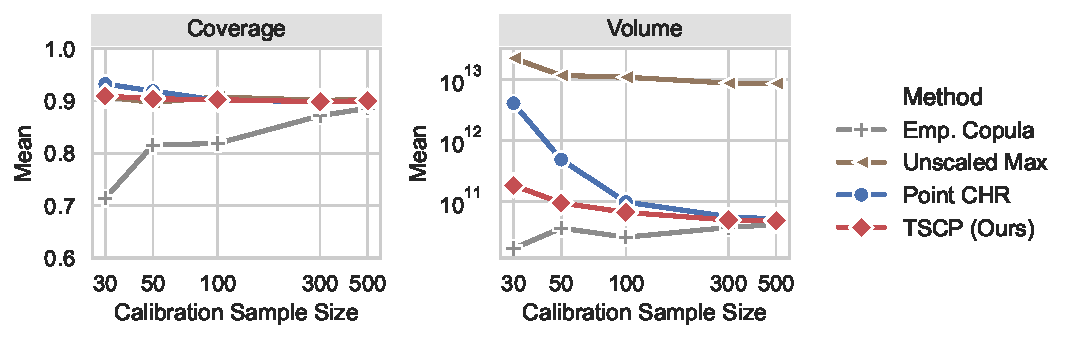
\includegraphics[width=0.9\textwidth]{figures/baselines/gaussian_10d.pdf} 
\caption{Average performance of the proposed TSCP method and alternative conformal prediction approaches on simulated data with $d=10$ outcome variables and heterogeneous noise variances. The target coverage level is $90\%$. TSCP consistently attains near-nominal coverage while producing the smallest prediction sets on average. Numerical results and corresponding standard deviations are reported in Table~\ref{tab:gaussian-heter}. }
     \label{fig:gaussian-heter}
\end{figure}


TSCP has near-nominal empirical coverage across calibration sizes and
smaller volumes than Point CHR and Unscaled Max. The volume penalty for
Point CHR is particularly pronounced when $n<100$, where its additional
split reduces the observations available for calibration. Unscaled Max
assigns one residual threshold to outputs with unequal noise scales and
therefore produces substantially larger rectangles. Emp. Copula yields
smaller regions but undercovers; its reuse of calibration observations for
dependence estimation precludes the split-conformal guarantee enjoyed by
the other benchmarks.


Figure~\ref{fig:gaussian-homo} reports results from analogous experiments in which the noise distribution has equal variance across dimensions, with $\epsilon^{\mathrm{homo}}_j \sim \mathcal{N}(0, 1)$ for all $j \in [10]$. This setting strongly favors the \emph{Unscaled Max} approach; nevertheless, our TSCP still performs as a close second.
Together, these two settings show that coordinate adaptation is useful when
noise scales differ, whereas unscaled calibration can be more efficient
when a common scale is appropriate.


\begin{figure}[!htbp]
    \centering
    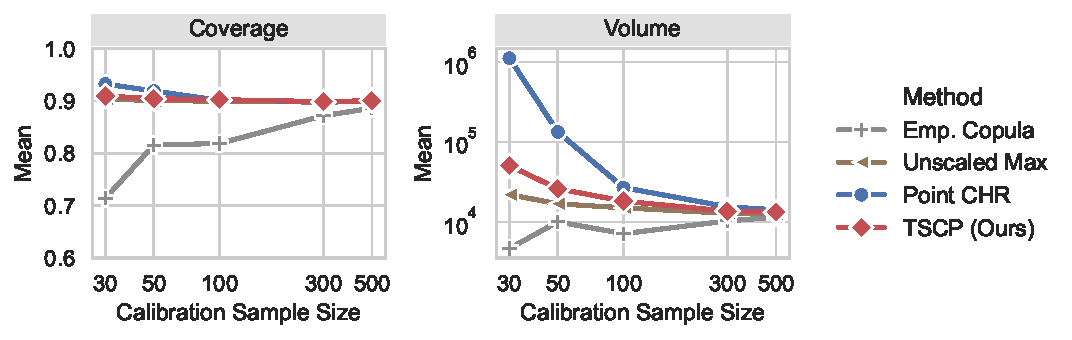
\includegraphics[width=0.9\textwidth]{figures/baselines/unit_gaussian_10d.pdf}
\caption{Average performance of the proposed TSCP method and alternative conformal prediction approaches in numerical experiments similar to those of Figure~\ref{fig:gaussian-heter}. Here, the outcome variables have homogeneous variance across their $d=10$ dimensions, which gives an advantage to the \emph{Unscaled Max} approach. The target coverage level is $0.9$. TSCP attains near-nominal coverage and is competitive, while Unscaled Max is the most efficient in this homogeneous setting. Numerical results and corresponding standard deviations are reported in Table~\ref{tab:gaussian-homo}.}
     \label{fig:gaussian-homo}
\end{figure}

The distributional comparisons below extend this analysis to Laplace,
mixture, and Gamma errors. The dependence and heterogeneity sweeps in
Appendices~\ref{app:dependence-sensitivity} and
\ref{app:heterogeneity-sensitivity} vary these features separately under
the independent-observation protocol.

\clearpage
\subsubsection{Distribution-Specific Tables}


Tables~\ref{tab:gaussian-heter}--\ref{tab:gamma} report coverage and
normalized residual-space volume for five noise laws. Gaussian errors
contrast unequal and equal coordinate scales; Laplace, mixture, and Gamma
errors vary the tail shape and symmetry under heterogeneous scaling.
The Laplace distributions are centered at zero, with the stated scale
parameter; the Gamma parameterization specifies shape followed by scale.

\subsubsection*{Gaussian Noise (heterogeneous)}

\begin{table}[H]
    \centering
    \input{figures/baselines/gaussian_10d_table}
    \caption{Performance of the proposed TSCP method and alternative conformal prediction approaches on simulated data with $d=10$ outcome variables, as in Figure~\ref{fig:gaussian-heter}. All results are averaged over $200$ trials with their one standard deviation reported in parenthesis.  
    The target coverage level is $0.9$. Coverage below this target is highlighted in \textcolor{red}{red}. For volume, lower is better. Smallest volume size (among those with valid theoretical coverage) is highlighted in \textbf{bold}. TSCP yields the tightest volume while maintaining valid coverage.}
    \label{tab:gaussian-heter}
\end{table}

\clearpage
\subsubsection*{Gaussian Noise (homogeneous)}

\begin{table}[H]
    \centering
    \input{figures/baselines/unit_gaussian_10d_table}
    \caption{Performance of the proposed TSCP method and alternative conformal prediction approaches on simulated data with $d=10$ outcome variables, as in Figure~\ref{fig:gaussian-homo}. Other details are as in Table~\ref{tab:gaussian-heter}. In this case, Unscaled Max yields the tightest volume while maintaining valid coverage, while TSCP remains a competitive second. }
    \label{tab:gaussian-homo}
\end{table}

\clearpage
\subsubsection*{Laplace Noise}
\begin{table}[H]
    \centering
    \input{figures/baselines/laplace_10d_table}
    \caption{Performance of the proposed TSCP method and alternative conformal prediction approaches on simulated data with $d=10$ outcome variables, and noise following a \emph{Laplace} distribution; i.e., $\epsilon _j \sim \mathrm{Laplace}(10-j+1)$ for all $j \in [10]$. Other details are as in Table~\ref{tab:gaussian-heter}.}
    \label{tab:laplace}
\end{table}

\clearpage
\subsubsection*{Mixture Noise}

\begin{table}[H]
    \centering
    \input{figures/baselines/mixed_10d_table}
    \caption{Performance of the proposed TSCP method and alternative conformal prediction approaches on simulated data with $d=10$ outcome variables, and noise following a \emph{Mixture} distribution; i.e., $\epsilon_j \sim \frac{1}{2}\mathrm{Laplace}(10-j+1)+\frac{1}{2}\mathcal{N}(0, (10-j+1)^2)$ for all $j \in [10]$. Other details are as in Table~\ref{tab:gaussian-heter}.}
    \label{tab:mixed}
\end{table}

\clearpage
\subsubsection*{Gamma Noise}
 
\begin{table}[H]
    \centering
    \input{figures/baselines/gamma_10d_table}
    \caption{Performance of the proposed TSCP method and alternative conformal prediction approaches on simulated data with $d=10$ outcome variables, and noise following a \emph{Gamma} distribution; i.e., $\epsilon_j \sim  \mathrm{Gamma}(1, 10-j+1)$ for all $j \in [10]$. Other details are as in Table~\ref{tab:gaussian-heter}.}
    \label{tab:gamma}
  \end{table}

\FloatBarrier
\subsection{Dependence Strength}
\label{app:dependence-sensitivity}

We vary the equicorrelation of the Gaussian noise over
$\rho\in\{0,0.3,0.6,0.9\}$ while retaining marginal standard deviations
$(10,9,\ldots,1)$ and a calibration size of $n=100$. Figure~\ref{fig:app-dependence}
shows that TSCP's empirical joint coverage is stable across this range:
$0.905$, $0.905$, $0.907$, and $0.908$, respectively. Its average
residual-space volume decreases from $6.37\times10^{10}$ at $\rho=0$ to
$9.47\times10^9$ at $\rho=0.9$. Point CHR and Unscaled Max also remain close
to the target. Emp. Copula improves as the correlation strengthens but remains
below the nominal level throughout the sweep. The experiment therefore does
not indicate a coverage failure of TSCP under strong equicorrelation, while
also showing that dependence materially changes region size.

\begin{figure*}[!htbp]
  \centering
  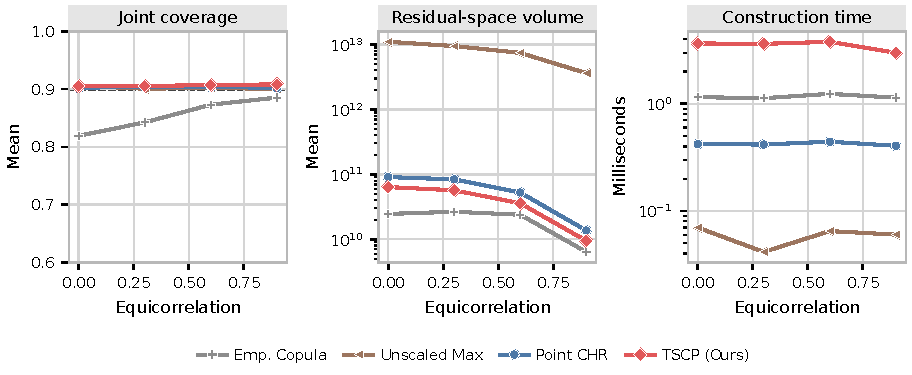
\includegraphics[width=0.92\textwidth]{figures/fig_app_dependence_sensitivity.pdf}
  \caption{Sensitivity to equicorrelated Gaussian noise at $d=10$ and
  $n=100$. The three panels report joint coverage, mean residual-space
  volume, and mean construction time. Results average 200 repetitions; the
  dashed line marks the target coverage.}
  \label{fig:app-dependence}
\end{figure*}

\FloatBarrier
\subsection{Severity of Coordinate Heterogeneity}
\label{app:heterogeneity-sensitivity}

To isolate heterogeneity across outcomes, we use independent Gaussian noise
and choose ten coordinate scales geometrically spaced between $r$ and $1$,
where $r\in\{1,2,5,10,20\}$. The calibration size is fixed at $n=100$.
Figure~\ref{fig:app-heterogeneity} shows that the coverage of TSCP, Point CHR,
and Unscaled Max is essentially unchanged as $r$ grows. At $r=1$, Unscaled
Max is slightly smaller than TSCP, with mean volumes $1.43\times10^4$ and
$1.80\times10^4$. At $r=20$, their mean volumes are
$3.44\times10^{15}$ and $5.75\times10^{10}$, respectively. This widening gap
is the expected benefit of coordinate adaptation: a single maximum-residual
threshold becomes increasingly inefficient when one scale must be used for
all coordinates. Emp. Copula remains smaller but has average coverage about
$0.821$ in this experiment.

\begin{figure*}[!htbp]
  \centering
  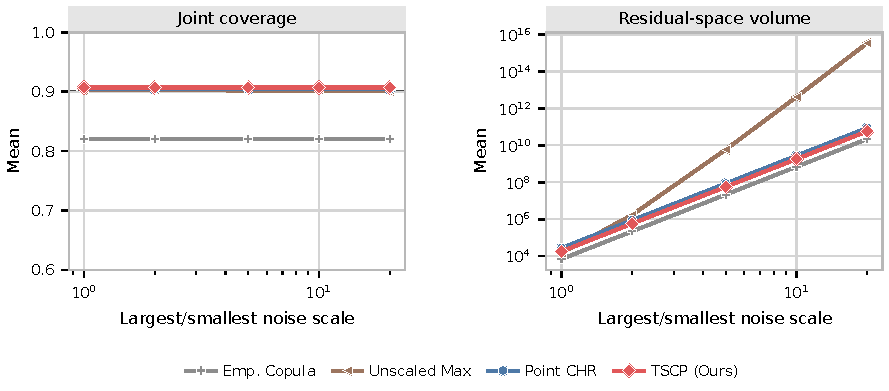
\includegraphics[width=0.84\textwidth]{figures/fig_app_heterogeneity_sweep.pdf}
  \caption{Sensitivity to the ratio between the largest and smallest outcome
  noise scales, with independent Gaussian errors and $n=100$. The scales are
  geometrically spaced, and both axes of the volume panel are logarithmic.
  Results average 200 repetitions.}
  \label{fig:app-heterogeneity}
\end{figure*}

\FloatBarrier
\subsection{Target Level and Small Calibration Samples}
\label{app:alpha-small-sample}

Figure~\ref{fig:app-alpha} repeats the dependent Gaussian experiment at
nominal coverage levels $0.8$, $0.9$, and $0.95$, with $n=100$ and
$\rho=0.6$. TSCP achieves empirical coverages $0.811$, $0.907$, and $0.954$.
As expected, increasing the target level increases all region volumes. The
relative ordering is stable: TSCP is smaller than Point CHR and dramatically
smaller than Unscaled Max, while Emp. Copula is smaller but below the nominal
coverage at every displayed target.

\begin{figure*}[!htbp]
  \centering
  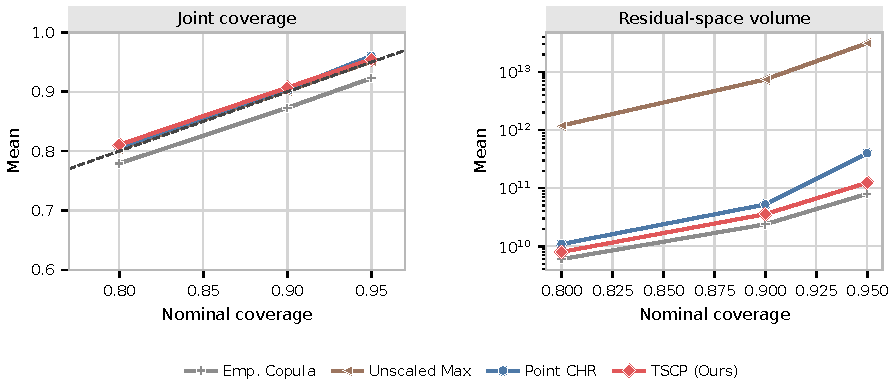
\includegraphics[width=0.84\textwidth]{figures/fig_app_alpha_sensitivity.pdf}
  \caption{Sensitivity to the nominal coverage level in the $d=10$
  equicorrelated Gaussian experiment with $n=100$ and $\rho=0.6$. The dashed
  diagonal in the left panel is exact nominal calibration. Results average
  200 repetitions.}
  \label{fig:app-alpha}
\end{figure*}

We separately examine $n\in\{10,20,30,50,100\}$ under independent Gaussian
noise. Figure~\ref{fig:app-small-calibration} distinguishes finite volumes
from the frequency of infinite output. At $n=10$, Point CHR has coverage one
and infinite volume in every repetition. This is a finite-sample quantile
effect, not evidence of a superior region: Point CHR divides the calibration
sample and its final subset is too small to supply a finite $0.9$ conformal
quantile. Point CHR is finite in all repetitions once $n\geq20$. TSCP and
Unscaled Max are finite throughout; both are conservative at the smallest
sample sizes, as expected from the discrete conformal rank. Emp. Copula
severely undercovers when $n$ is small because it estimates dependence and
calibrates on the same limited sample.

\begin{figure*}[!htbp]
  \centering
  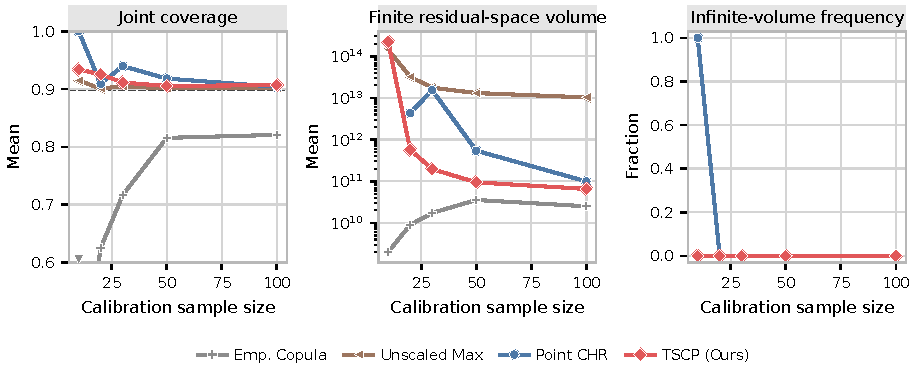
\includegraphics[width=0.92\textwidth]{figures/fig_app_small_calibration.pdf}
  \caption{Small-calibration-sample stress test with independent Gaussian
  noise and scales $(10,9,\ldots,1)$. The middle panel averages only finite
  residual-space volumes; the right panel reports the fraction of repetitions
  with infinite volume. A downward triangle at the lower plotting boundary
  marks the Emp. Copula mean below $0.6$. Results average 200 repetitions.}
  \label{fig:app-small-calibration}
\end{figure*}

\FloatBarrier
\subsection{Heavy-Tailed Noise and the Role of Moment Conditions}
\label{app:heavy-tails}

We examine independent Student $t$ noise with
$d=10$, a common unit scale across coordinates, and degrees of freedom
$\nu\in\{1.5,2,3\}$. The cases $\nu=1.5$ and $\nu=2$ have infinite variance
and therefore lie outside Assumption~\ref{eq:assumption-scores}, which is
invoked by the validity theorem as well as the moment-based motivation;
$\nu=3$ has finite variance but remains heavy-tailed. These results should be
read as an empirical stress test, not as an extension of the stated
theory to infinite-variance distributions.

\subsubsection{Independent-Observation Evaluation}
Figure~\ref{fig:app-heavy-tails} uses the independent-observation protocol
of Appendix~\ref{app:experimental-protocols}.

TSCP remains near the target in the displayed cases. For example, at $n=30$
its coverages are $0.909$, $0.908$, and $0.912$ as $\nu$ increases, while at
$n=500$ they are $0.898$, $0.901$, and $0.900$. Efficiency is much less
stable. At $n=30$, the mean TSCP volume falls from $1.59\times10^{20}$ for
$\nu=1.5$ to $5.92\times10^{13}$ for $\nu=3$; at $n=500$, it falls from
$8.42\times10^{13}$ to $6.07\times10^7$. The explosive volumes make clear
that empirical coverage alone is not evidence of practically useful behavior
under very heavy tails.

\begin{figure*}[!htbp]
  \centering
  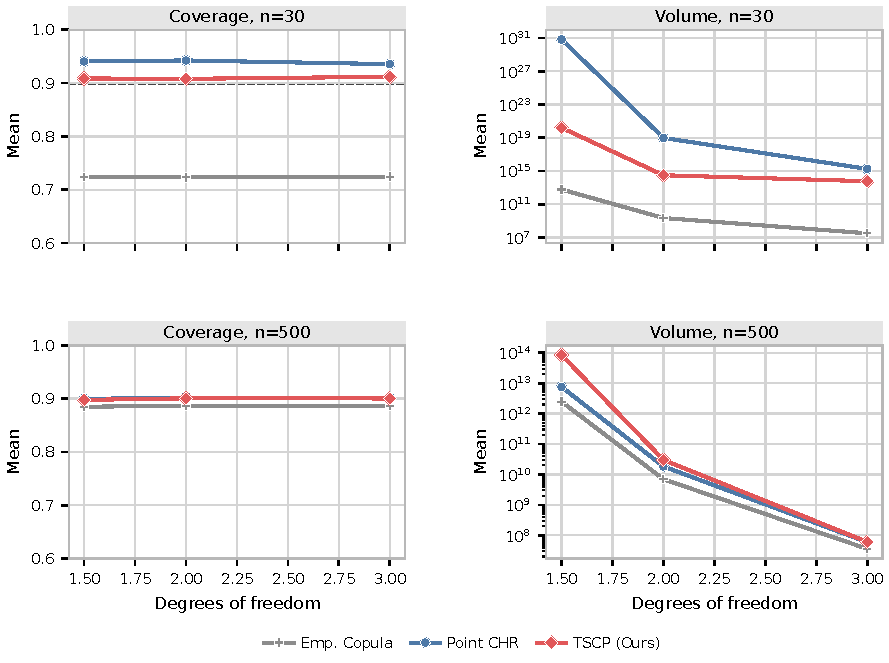
\includegraphics[width=0.86\textwidth]{figures/fig_app_heavy_tail_stress.pdf}
  \caption{Coverage and mean residual-space volume under independent,
  common-scale Student $t$ noise for $d=10$. The top row uses $n=30$
  calibration examples and the bottom row uses $n=500$. Results average 200
  repetitions; volume is shown on a logarithmic scale.}
  \label{fig:app-heavy-tails}
\end{figure*}

\FloatBarrier
\subsubsection{Fixed-Pool Evaluation} \label{app:hevy_tailed_simulation}


Figure~\ref{fig:t} evaluates the same unit-scale Student's-$t$ noise family
with $d=10$, $\mathrm{DF}\in\{1.5,2,3\}$, and calibration sizes
$n\in\{30,500\}$ under the fixed-pool protocol. Results average 200
repetitions. Coverage remains near the target while interval volumes grow
substantially as the degrees of freedom decrease. Point CHR is less
efficient at the smaller calibration size but can outperform TSCP at the
larger size. As in the independent-observation evaluation, the
infinite-variance cases lie outside Assumption~\ref{eq:assumption-scores}
and do not extend the coverage theorem.


\begin{figure}[!htbp]
     \centering
     \begin{subfigure}[b]{\textwidth}
         \centering
         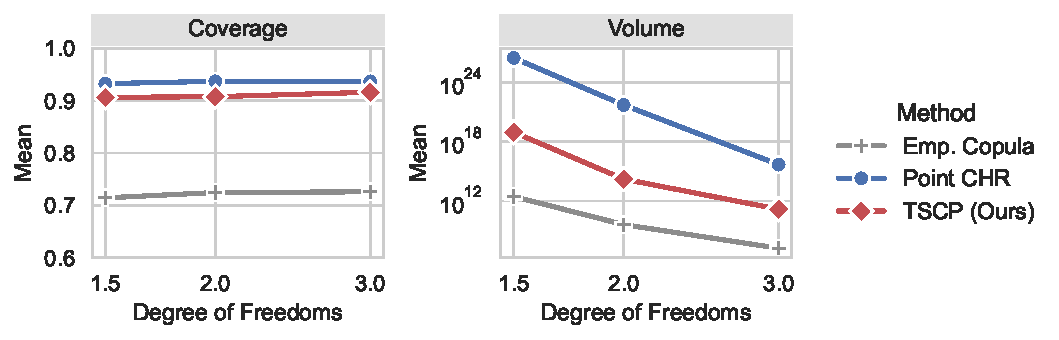
\includegraphics[width=0.9\textwidth]{figures/t/t_n30_10d.pdf}
         \caption{Small sample, $|\mathcal{D}_{\mathrm{cal}}|=30$. Output dimensions $d=10$.}
         \label{fig:t-n30-10d}
     \end{subfigure}
     \vfill
     \begin{subfigure}[b]{\textwidth}
         \centering
         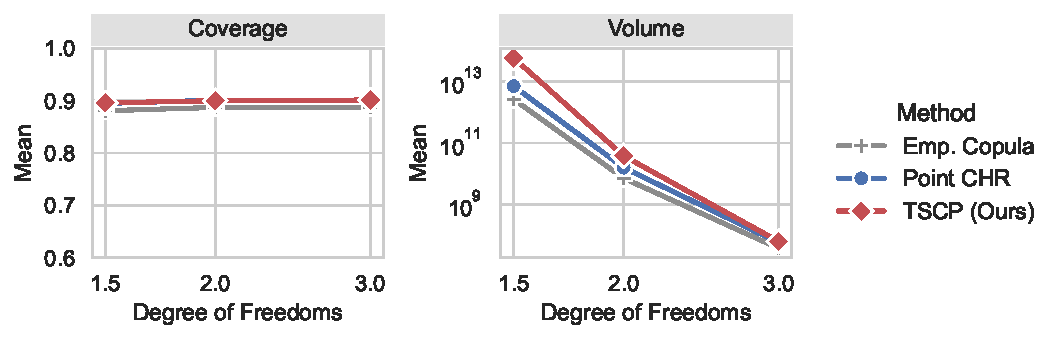
\includegraphics[width=0.9\textwidth]{figures/t/t_n500_10d.pdf}
         \caption{Large sample, $|\mathcal{D}_{\mathrm{cal}}|=500$. Output dimensions $d=10$.}
         \label{fig:t-n500-10d}
     \end{subfigure}
        \caption{Performance of the proposed TSCP method and other approaches on simulated data with noise following a Student's-$t$ distribution with varying degrees of freedom, using small (a) and large (b) sample sizes. The target coverage level is 0.9. All methods except \emph{Emp.~Copula} have near-nominal coverage in all settings. TSCP has near-nominal empirical coverage in these displayed heavy-tail cases; the infinite-variance cases are outside the stated assumptions. In the small sample setting, Point CHR suffers more in terms of prediction set size due to its inefficient use of calibration data, although it can outperform TSCP in large samples.}
        \label{fig:t}
\end{figure}
 
% \begin{table}
%     \centering
%     \input{figures/t/t_n30_10d}
%     \caption{Performance on Student's-$t$ distribution with varying degree of freedoms on small sample size $|\mathcal{D}_{\mathrm{cal}}|=30$. This table contains all data used to generate Figure~\ref{fig:t-n30-10d} along with one standard deviation of the test coverage and volume over $200$ trials. Target coverage is $0.9$. Coverage below this target is highlighted in \textcolor{red}{red}. For volume, lower is better. Smallest volume size (among those with valid coverage) is highlighted in \textcolor{red}{red}. }
%     \label{tab:t-n30-10d}
% \end{table}

% \begin{table}
%     \centering
%     \input{figures/t/t_n500_10d}
%     \caption{Performance on Student's-$t$ distribution with varying degree of freedoms on large sample size $|\dataset_{\mathrm{cal}}|=500$. This table contains all data used to generate Figure~\ref{fig:t-n500-10d} along with one standard deviation of the test coverage and volume over $200$ trials. Target coverage is $0.9$. Coverage below this target is highlighted in \textcolor{red}{red}. For volume, lower is better. Smallest volume size (among those with valid coverage) is highlighted in \textcolor{red}{red}. Point CHR has the smallest volume while maintaing valid coverage when the degree of freedom is less than $3$, but when systematic outliers getting removed as the degree of freedom increases, our TSCP becomes the one with the smallest volume while maintaining valid coverage. }
%     \label{tab:t-n500-10d}
% \end{table}



\FloatBarrier
\subsection{Exchangeable Contamination Stress Test}
\label{app:contamination}

To test sensitivity to atypically large residuals, we contaminate the
Gaussian experiment at rates
$\varepsilon\in\{0,0.01,0.05,0.10\}$. Independently for each observation, all
ten noise coordinates are multiplied by $10$ with probability $\varepsilon$;
the same exchangeable mechanism is used for training, calibration, and test
data. The calibration size is $n=100$. We report median rather than mean
volume because the contaminated distribution produces a small number of
extreme regions.

Figure~\ref{fig:app-contamination} shows that TSCP coverage changes from
$0.904$ without contamination to $0.902$ at $10\%$ contamination, but its
median volume grows from $5.38\times10^{10}$ to $1.10\times10^{17}$. Point CHR
and Unscaled Max exhibit the same qualitative inflation, and Emp. Copula
under-covers at every contamination level. Thus, the conformal calibration is
comparatively stable in coverage, whereas the sample mean and standard
deviation used for coordinate scaling are not robust efficiency summaries.
Replacing them by robust estimators would change the construction and its
analysis and requires a separate validity argument.

\begin{figure*}[!htbp]
  \centering
  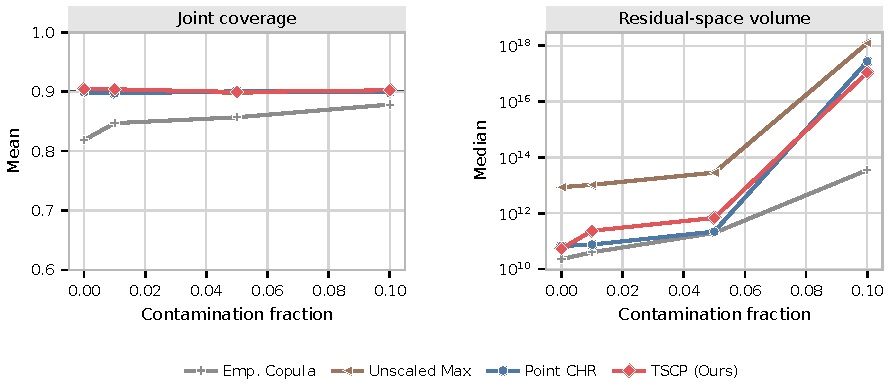
\includegraphics[width=0.84\textwidth]{figures/fig_app_contamination_stress.pdf}
  \caption{Row-wise contamination stress test with $d=10$ and $n=100$. A
  contaminated observation has every noise coordinate multiplied by $10$.
  The right panel reports median residual-space volume over 200 repetitions
  on a logarithmic scale.}
  \label{fig:app-contamination}
\end{figure*}

\FloatBarrier
\subsection{Additional CQR Sensitivity Analyses}
\label{app:cqr-sensitivity}

\paragraph{Base-interval width.}
The main CQR comparison uses base-interval miscoverage $0.5$. We repeat it at
$0.3$, $0.5$, $0.7$, and $0.9$, fixing $n=100$ and final miscoverage $0.1$.
Figure~\ref{fig:app-cqr-base} shows that capped-score TSCP has empirical
coverage between $0.903$ and $0.906$ and mean outcome-space volume between
$2.80\times10^4$ and $3.77\times10^4$ across the sweep. Unscaled Max behaves
similarly, while Emp. Copula undercovers. CQHR remains close to nominal
coverage but its volume is highly sensitive to the fitted base interval in
this design. The result supports using the moderate $0.5$ base interval for
the primary comparison and cautions against drawing conclusions from one
extreme base-quantile choice.

\begin{figure*}[!htbp]
  \centering
  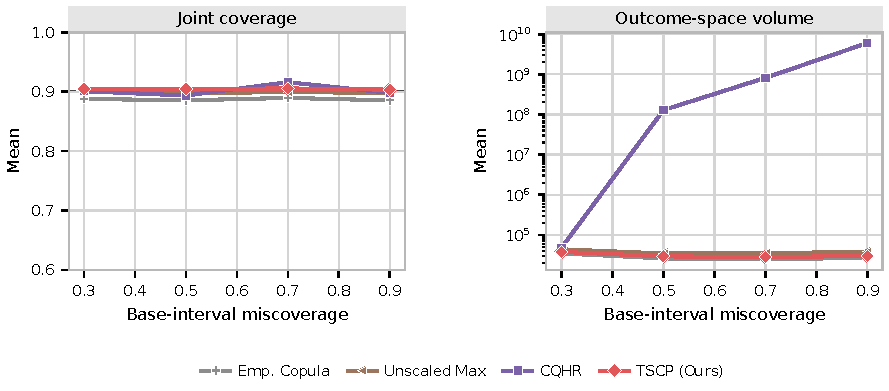
\includegraphics[width=0.84\textwidth]{figures/fig_app_cqr_base_interval.pdf}
  \caption{CQR sensitivity to the base-interval miscoverage with $d=3$,
  $n=100$, and final target coverage $0.9$. TSCP uses capped scores, CQHR uses
  its native construction, and results average 30 independent repetitions.}
  \label{fig:app-cqr-base}
\end{figure*}

\paragraph{Shifted scores.}
An alternative way to enforce nonnegativity is to replace the signed CQR score
$S_j$ by $S_j+C$, apply TSCP, and subtract $C$ from the final coordinate
adjustment. We test $C\in\{100,300,1000\}$. As shown in
Figure~\ref{fig:app-cqr-shift}, the recorded TSCP rectangle is invariant to
$C$ in this range up to numerical roundoff and agrees exactly, to recorded numerical precision, with
the TSCP-GWC rectangle: the maximum coordinate-length difference is zero in
all 30 repetitions for every $C$. Consequently, this experiment does not
identify a practically meaningful shift constant and the shifted construction
does not provide a distinct local refinement in this design. This is an
empirical finding, not a translation-invariance theorem for arbitrary data.
A fixed shift is justified by a bound on the score over the relevant input
domain, not only its observed calibration minimum: for ordered base intervals
of width $w_j(x)$, $S_j(x,y)\geq-w_j(x)/2$, so a known uniform width bound
$w_j(x)\leq M$ gives the sufficient choice $C\geq M/2$. The experiment uses
fixed constants and is not a general selector for $C$. The primary comparison
uses capped nonnegative scores; the fixed-constant sweep
does not supply a data-adaptive tuning rule for $C$.

\begin{figure*}[!htbp]
  \centering
  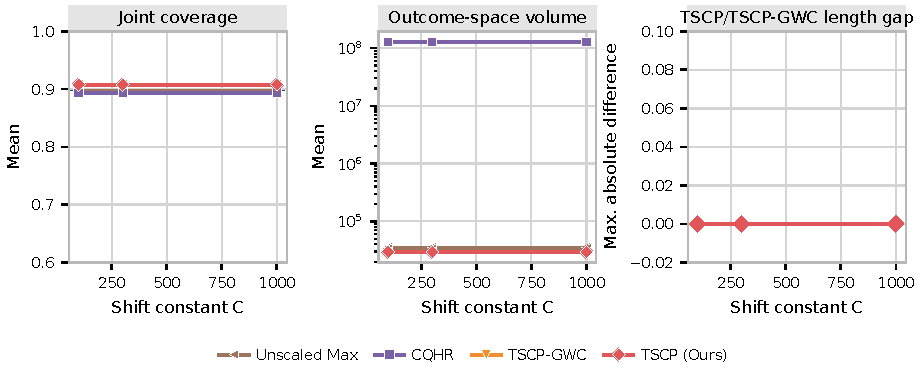
\includegraphics[width=0.92\textwidth]{figures/fig_app_cqr_shift_sensitivity.pdf}
  \caption{Sensitivity of shifted CQR scores to the additive constant $C$.
  The first two panels report coverage and mean outcome-space volume; the
  third reports the maximum coordinate-length difference between shifted TSCP
  and TSCP-GWC. Results use $d=3$, $n=100$, and 30 independent repetitions.}
  \label{fig:app-cqr-shift}
\end{figure*}

\FloatBarrier
\subsection{Low-Dimensional Shape-Template Baseline}
\label{app:shape-template}

We compare with the convex shape-template approach of
\citet{tumu2024templates}. We use the public \texttt{conformal-region-designer} components:
a kernel density estimate on a grid of size $20$ per dimension, mean-shift
clustering, and an axis-aligned hyperrectangular template. The signed
calibration residuals are divided equally between fitting the density and
template and conformalizing its inflation. We use a score-consistent
hyperrectangle implementation and impose an aspect-ratio floor of $0.05$ when
a very small fitted cluster is degenerate along one coordinate. This detail
keeps the conformal inflation finite and is stated here because it differs
from calling the released rectangle class without modification.

We use $d=2$ with independent Gaussian scales $(2,1)$ and calibration
sizes $n\in\{30,50,100,200\}$. Shape-template volume is divided by $2^d$ to match
the residual-space volume convention used for the symmetric rectangular
methods. Figure~\ref{fig:app-shape-template} shows broadly comparable coverage.
At $n=100$, the shape-template method has coverage $0.904$, mean normalized
volume $10.07$, and mean construction time $98.7$ milliseconds; TSCP has
coverage $0.906$, mean volume $8.04$, and mean construction time $0.80$
milliseconds. For each sample size shown, TSCP has a smaller mean normalized
volume. Its construction time is also over two orders of magnitude shorter
for this implementation.

This is deliberately a low-dimensional comparison. A Cartesian KDE grid has
$20^d$ locations and is therefore not computationally meaningful at the
$d=10$ scale of the main synthetic experiment. The experiment establishes a
comparison with a flexible convex template where the released computational
strategy is applicable; it is not evidence that either method dominates all
shape-template choices in higher dimensions.

\begin{figure*}[!htbp]
  \centering
  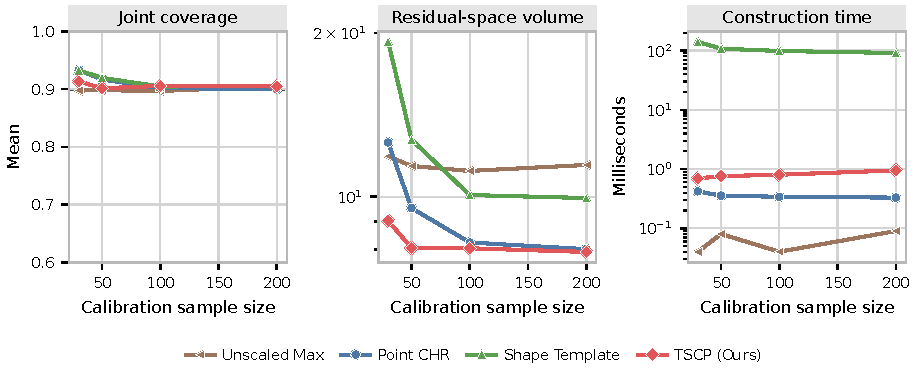
\includegraphics[width=0.92\textwidth]{figures/fig_app_shape_template_baseline.pdf}
  \caption{Comparison with a KDE/mean-shift hyperrectangular shape template
  for $d=2$ Gaussian residuals with scales $(2,1)$. Volume follows the same
  $2^{-d}$ normalization as the other residual-space experiments. Results
  average 100 independent repetitions, and runtime excludes the common
  regression fit.}
  \label{fig:app-shape-template}
\end{figure*}

\FloatBarrier
\subsection{Oracle Approximation and Computational Scaling}
\label{app:ours_simulation}

These comparisons use the fixed-pool protocol
in Appendix~\ref{app:experimental-protocols}.

The additional methods considered in this section include (i) \emph{Naive}, the heuristic plug-in rescaling method that uses location and scale parameters estimated directly from the calibration data without further adjustments, summarized in Algorithm~\ref{alg:std-plug-in}; (ii) \emph{TSCP-S}, the inefficient data-splitting variant summarized in Algorithm~\ref{alg:std-ds}; (iii) \emph{TSCP-GWC}, our conservative global-worst-case method summarized in Algorithm~\ref{alg:global}; (iv) \emph{TSCP-LWC}, the aggregated union described in Section~\ref{sec:method-lwc} but not enclosed by a rectangle. 


\begin{figure}[!htbp]
    \begin{subfigure}[b]{\textwidth}
        \centering
        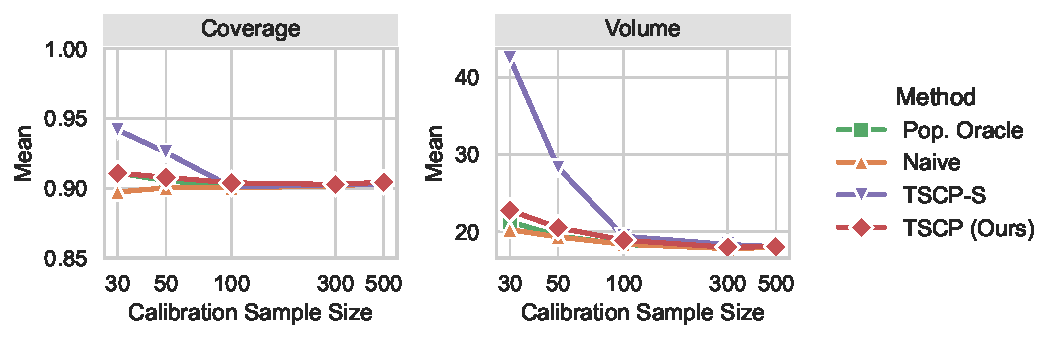
\includegraphics[width=0.9\textwidth]{figures/ours/ours_approximation_2d.pdf}
    \end{subfigure}
    \begin{subfigure}[b]{\textwidth}
        \centering
        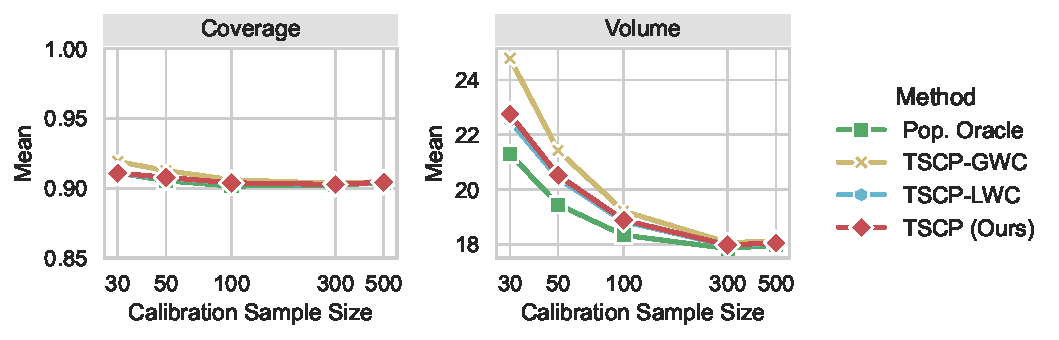
\includegraphics[width=0.9\textwidth]{figures/ours/ours_containment_2d.pdf}
    \end{subfigure}
    \caption{Performance of TSCP and alternative approaches on simulated data with $d=2$ targets and heterogeneous Laplace noise. The target coverage level is $90\%$. Results are averaged over $200$ trials. All methods achieve near-nominal coverage and approximate \emph{Pop.~Oracle} as the calibration sample size increases. TSCP tracks TSCP-LWC closely, with an almost indistinguishable average volume, highlighting the tightness of its rectangular enclosure.}
    \label{fig:approximation1}
\end{figure}

All methods compared in Figure~\ref{fig:approximation1} tend to approximate \emph{Pop.~Oracle} well as $n$ increases, with TSCP and TSCP-LWC being the two most stable and fastest approximations among all methods with theoretical coverage. These results also show that TSCP encloses the aggregated union TSCP-LWC very tightly, and that TSCP-GWC is conservative, though it still performs better than the data-splitting variant TSCP-S. Despite lacking a finite-sample coverage guarantee, the \emph{Naive} approach performs well, as also shown in Figure~\ref{fig:approximation2}.

\begin{figure}[!htbp]
    \centering
    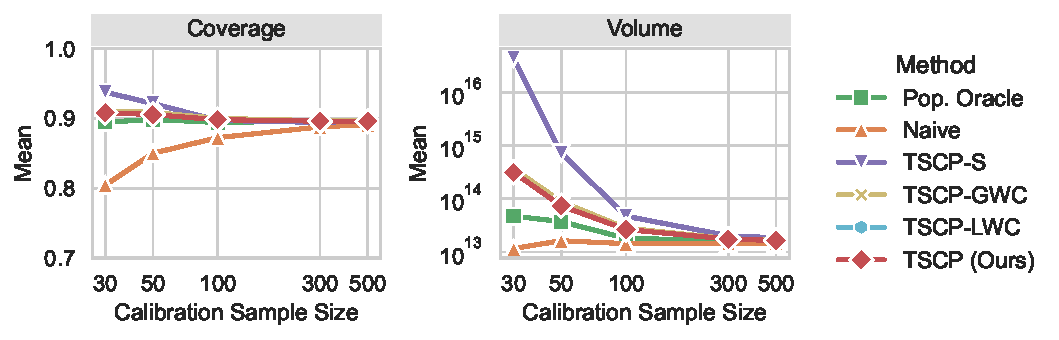
\includegraphics[width=0.9\textwidth]{figures/ours/ours_containment_10d.pdf}
    \caption{Performance of TSCP and alternative approaches on simulated data with $d=10$ targets. Other details are as in Figure~\ref{fig:approximation1}. TSCP-LWC is omitted from this figure due to its prohibitive cost with even moderately high-dimensional outcomes.}
    \label{fig:approximation2}
\end{figure}

Figure~\ref{fig:runtime} better highlights the prohibitive computational cost of TSCP-LWC, by reporting on the results of similar experiments where a small sample size is fixed, $|\mathcal{D}_{\mathrm{cal}}|=30$, while the outcome dimensions are gradually increased: $d \in \{2, 3, 4, 5, 10, 20, 30\}$.

\begin{figure}[!htbp]
    \centering
    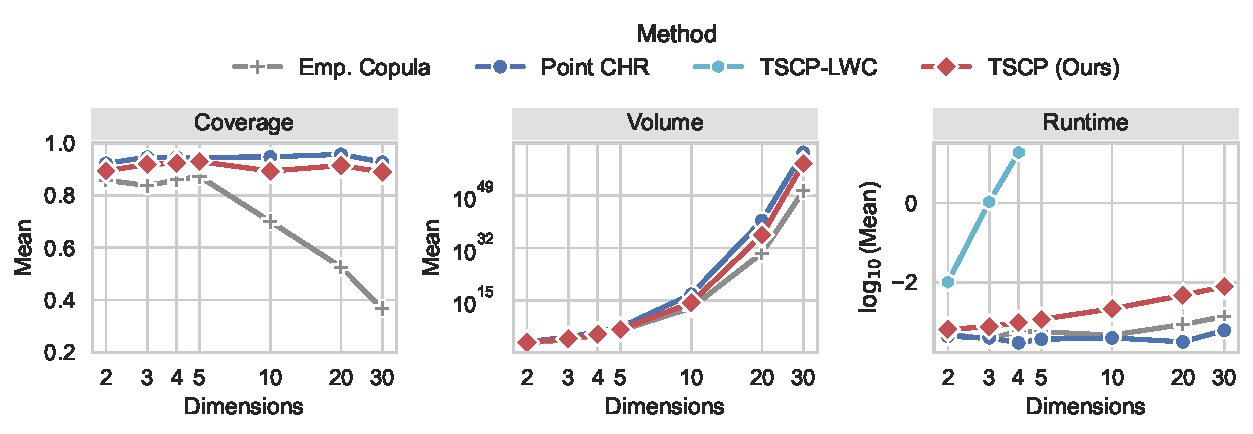
\includegraphics[width=\textwidth]{figures/ours/ours_runtime.pdf}
    \caption{Performance of TSCP and alternative approaches on simulated data with fixed sample size $|\mathcal{D}_{\mathrm{cal}}|=30$, as a function of the number of output dimensions $d$. Other details are as in Figure~\ref{fig:approximation1}. These results are averaged over $30$ repetitions under the fixed-pool protocol. The runtime results are presented in seconds on a $\log_{10}$ scale. 
    The runtime of all methods except TSCP-LWC scales well with number of dimensions. TSCP-LWC is only applied when $d \in \{2,3,4\}$ due to the exponential growth of its runtime. }
    \label{fig:runtime}
\end{figure}

\FloatBarrier
\subsection{Real-Data Coverage and Efficiency}
\label{app:real-coordinate-audit}

\subsubsection{Dataset-Level Coverage and Volume}

Table~\ref{tab:real} presents dataset-level coverage and normalized volume
for the benchmark evaluation in Section~\ref{sec:real-data-experiments},
including the across-split standard deviations. Each dataset uses 200
random $75\%/5\%/20\%$ training/calibration/test splits, with multitask
lasso at regularization $10^{-4}$ on \texttt{stock} and random forests
elsewhere. The four larger benchmark datasets follow related multivariate
regression studies \citep{pmlr-v258-park25c,dheur2025unified}; the
\texttt{student} and \texttt{energy} datasets emphasize smaller
calibration samples.

TSCP's volume advantage on four of the six datasets coexists with larger
volumes than Point CHR on \texttt{rf2} and Unscaled Max on
\texttt{student}. Point CHR's additional split makes its final
\texttt{stock} calibration sample too small for a finite $0.9$ conformal
quantile. Emp. Copula undercovers on these datasets. The coordinate-level
analysis below examines how such joint-coverage and volume comparisons
relate to the informativeness of individual intervals.

\begin{table}[!htbp]
\centering
\captionsetup[subtable]{justification=centering}
\small
\begin{subtable}{\textwidth}
\centering
\begin{tabular}[t]{l c c c c }
\toprule
\textbf{Method} & \multicolumn{2}{c}{Stock $(d=6,\, n=15)$} & \multicolumn{2}{c}{rf2 $(d=8,\, n=384)$} \\
\cmidrule(lr){2-3}\cmidrule(lr){4-5}
& Coverage & Volume & Coverage & Volume \\
\midrule
Unscaled Max & 0.940(0.057) & 6.03e-02(1.57e-01) & 0.900(0.016) & 4.14e+03(2.90e+03) \\
Emp. copula & \color{red}0.727(0.113) & 1.01e-05(9.80e-06) & \color{red}{0.893(0.016)} & 5.35e+01(4.69e+01) \\
Point CHR & 1.000(0.000) & \text{inf} & 0.901(0.022) & \textbf{{6.85e+01(7.55e+01)}} \\
TSCP & 0.956(0.059) & \textbf{{1.86e-03(8.55e-03)}} & 0.901(0.017) & 5.42e+02(1.50e+03) \\
\midrule

\end{tabular}
%\subcaption{First panel: Stock, rf2.}
\end{subtable}

\small
\begin{subtable}{\textwidth}
\centering
\begin{tabular}[t]{l c c c c }
\midrule
\textbf{Method} & \multicolumn{2}{c}{scm1d $(d=16,\, n=490)$} & \multicolumn{2}{c}{scm20d $(d=16,\, n=448)$} \\
\cmidrule(lr){2-3}\cmidrule(lr){4-5}
& Coverage & Volume & Coverage & Volume \\
\midrule
Unscaled Max & 0.900(0.016) & 2.74e+39(4.02e+39) & 0.901(0.016) & 2.70e+40(2.92e+40) \\
Emp. copula & \color{red}{0.893(0.016)} & 1.09e+39(1.34e+39) & \color{red}{0.892(0.017)} & 1.178e+40(1.190e+40) \\
Point CHR & 0.905(0.020) & 2.84e+39(5.43e+39) & 0.902(0.023) & 3.00e+40(8.00e+40) \\
TSCP & 0.901(0.015) & \textbf{{1.52e+39(2.61e+39)}} & 0.901(0.016) & \textbf{{1.53e+40(1.50e+40)}} \\
\midrule

\end{tabular}
%\subcaption{Second panel: scm1d, scm20d.}
\end{subtable}

\small
\begin{subtable}{\textwidth}
\centering
\begin{tabular}[t]{l c c c c }
\midrule

\textbf{Method} & \multicolumn{2}{c}{Energy $(d=2,\, n=38)$} & \multicolumn{2}{c}{Student $(d=3,\, n=32)$} \\
\cmidrule(lr){2-3}\cmidrule(lr){4-5}
& Coverage & Volume & Coverage & Volume \\
\midrule
Unscaled Max & 0.917(0.049) & 1.58e+01(6.80e+00) & 0.904(0.055) & \textbf{{1.51e+02(1.27e+02)}} \\
Emp. copula & \color{red}0.886(0.061) & 5.41e+00(4.49e+00) & \color{red}0.861(0.073) & 1.08e+02(7.19e+01) \\
Point CHR & 0.899(0.069) & 8.81e+00(2.42e+01) & 0.939(0.057) & 6.89e+02(1.07e+03) \\
TSCP & 0.922(0.048) & \textbf{{6.95e+00(4.43e+00)}} & 0.912(0.056) & 1.98e+02(1.77e+02) \\

\bottomrule
\end{tabular}
%\subcaption{Third panel: Energy, Student.}
\end{subtable}

\caption{Performance of the proposed TSCP method and alternative conformal prediction approaches on real datasets. Results are averaged over $200$ random splits of the data into training/calibration/and test subsets, with one standard deviation reported in parentheses. The target coverage level is $0.9$. Coverage values below the target are highlighted in \textcolor{red}{red}, and the smallest volume among methods achieving valid coverage is highlighted in \textbf{bold}.}
\label{tab:real}
\end{table}

\FloatBarrier

\subsubsection{Coordinate-Wise Coverage}
The coordinate-analysis batch in Section~\ref{sec:real-data-diagnostics}
uses the split proportions, calibration sizes, and model settings in
Section~\ref{sec:real-data-experiments}. In each of the 200 splits we record
full interval lengths and marginal test coverage for all 51 output
coordinates across the six datasets, for all four methods. Together this
gives 40,800 split--method--coordinate records. Comparisons are paired on
common fitted models and test observations.

Figure~\ref{fig:app-real-marginal-coverage} reports all coordinate-wise
coverage means, and Table~\ref{tab:real-diagnostic-coverage} reports the
matching joint coverage. The $0.9$ line is the joint target used for
calibration, not an assertion that every marginal should equal $0.9$.
For a rectangular region, each coordinate's empirical coverage is at least
the empirical joint coverage on the same test set, but the marginal rates
can differ substantially. Thus, shorter intervals in
Figure~\ref{fig:body-real-coordinate-bars} must be interpreted alongside
both kinds of coverage.

TSCP's mean joint coverages are $0.956$, $0.902$, $0.901$, $0.901$,
$0.923$, and $0.912$ on \texttt{stock}, \texttt{rf2}, \texttt{scm1d},
\texttt{scm20d}, \texttt{energy}, and \texttt{student}, respectively.
The target lies within one across-split standard deviation of each mean;
this is a variability diagnostic, not a confidence interval for the mean.
The coordinate means are not equal: for example, TSCP's marginal coverages
range from about $0.972$ to $0.999$ on \texttt{stock}, while its joint
coverage is $0.956$. On \texttt{energy}, the two marginal coverages are
$0.962$ and $0.954$, with joint coverage $0.923$. This illustrates why
interval-length allocation and marginal balance cannot be read off from a
single joint-coverage number.

\begin{table}[!htbp]
  \centering
  \small
  \begin{tabular}{lrrrr}
\toprule
Dataset & Emp.\ Copula & Unscaled Max & Point CHR & TSCP \\
\midrule
\texttt{stock} & $0.727\,(0.113)$ & $0.940\,(0.057)$ & $1.000\,(0.000)$ & $0.956\,(0.059)$ \\
\texttt{rf2} & $0.893\,(0.016)$ & $0.900\,(0.016)$ & $0.901\,(0.022)$ & $0.902\,(0.017)$ \\
\texttt{scm1d} & $0.893\,(0.016)$ & $0.900\,(0.016)$ & $0.905\,(0.020)$ & $0.901\,(0.015)$ \\
\texttt{scm20d} & $0.892\,(0.017)$ & $0.901\,(0.016)$ & $0.902\,(0.023)$ & $0.901\,(0.016)$ \\
\texttt{energy} & $0.887\,(0.061)$ & $0.917\,(0.048)$ & $0.899\,(0.069)$ & $0.923\,(0.048)$ \\
\texttt{student} & $0.861\,(0.073)$ & $0.904\,(0.055)$ & $0.939\,(0.057)$ & $0.912\,(0.056)$ \\
\bottomrule
\end{tabular}

  \caption{Joint test coverage for the real-data coordinate-analysis batch.
  Entries are the mean and one across-split standard deviation over 200
  splits. These measurements correspond to the interval lengths in
  Figure~\ref{fig:body-real-coordinate-bars} and the marginal coverages in
  Figure~\ref{fig:app-real-marginal-coverage}.}
  \label{tab:real-diagnostic-coverage}
\end{table}

\begin{figure}[!htbp]
  \centering
  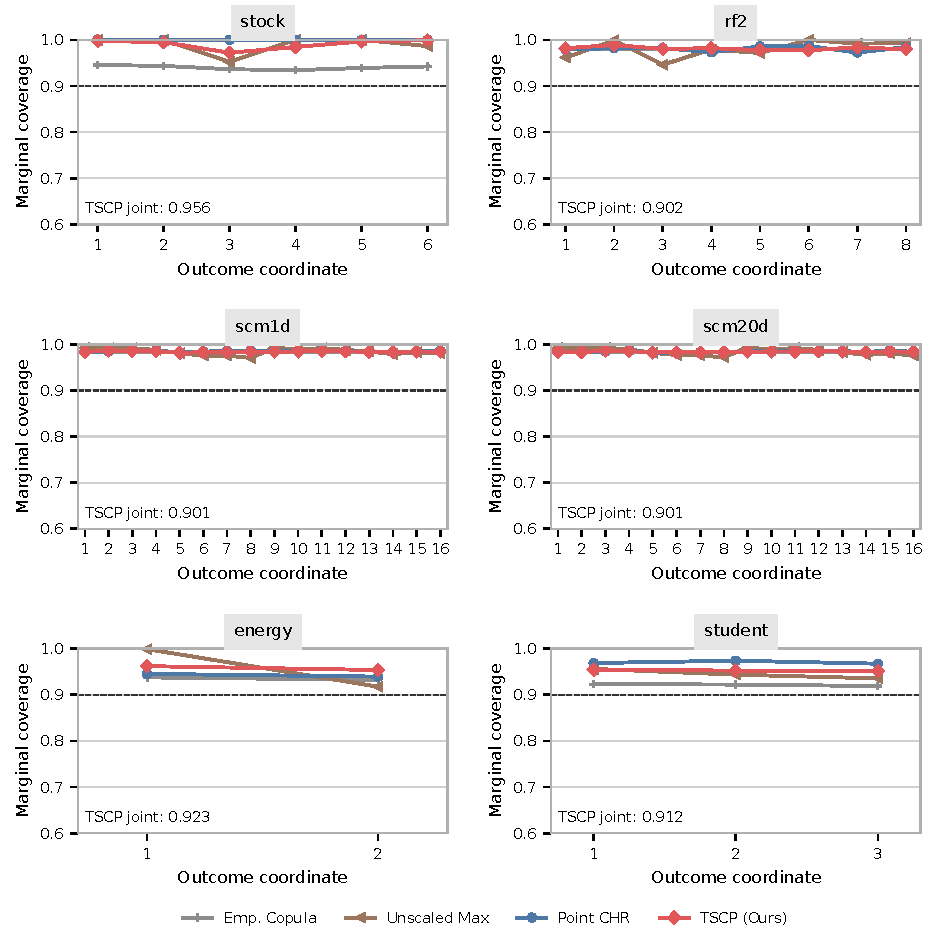
\includegraphics[width=0.96\textwidth]{figures/fig_app_real_marginal_coverage.pdf}
  \caption{Coordinate-wise marginal coverage over 200 splits of each
  real dataset. The dashed line is the $0.9$ joint target, and each panel
  also reports TSCP's mean joint coverage. Across-split standard deviations
  and pointwise Monte Carlo intervals are provided in the supplementary
  data. Coordinates follow the target-column order of each dataset.}
  \label{fig:app-real-marginal-coverage}
\end{figure}

Supplementary data include coordinate lengths, paired length ratios,
marginal and joint coverages, and across-split standard deviations.
Standard errors obtained by dividing
the across-split standard deviation by $\sqrt{200}$ quantify Monte Carlo
variation over randomized splits of each fixed dataset. They do not measure
uncertainty over independently sampled populations, and the reported
pointwise intervals are not simultaneous statements over all coordinates.

\FloatBarrier
\subsection{Search-Regime Sensitivity to the Target Level}
\label{app:real-search-stress}

To explore regimes beyond the main $90\%$ target, we reuse the same 200
calibration residual matrices per dataset and vary the miscoverage level over
$\alpha\in\{0.1,0.3,0.5,0.7,0.9\}$. This is a computational diagnostic,
not an additional $90\%$-coverage experiment: the nominal coverage changes
with $\alpha$. No model is refitted or selected based on the branch outcomes.
The sweep records 6,000 dataset--split--level configurations. It separates
runs entering any backward search from those taking the global fallback.

Unlike the main target, the sweep reaches both exceptional branches.
On \texttt{energy} at $\alpha=0.5$, backward search occurs in $3/200$
splits ($1.5\%$), while fallback occurs in $140/200$ ($70\%$). The
remaining 57 splits use only binary search. Mean whole-call times
conditional on these three regimes are $0.295$, $0.121$, and $0.268$ ms,
respectively. At $\alpha=0.7$ and $0.9$, 10 energy splits use backward
search and 190 fall back. In every observed backward-search case, each of
the two coordinates inspects only one backward candidate. These examples
therefore exercise the branch without exhibiting a long backward scan.

At $\alpha=0.9$, fallback counts are 139, 185, 180, 186, 190, and 200 out
of 200 for \texttt{stock}, \texttt{rf2}, \texttt{scm1d}, \texttt{scm20d},
\texttt{energy}, and \texttt{student}, respectively. No backward search
is observed in the other five datasets over the displayed levels.
Fallback is often faster because it returns the already computed global
rectangle, so a lower average runtime at an extreme target need not
indicate a more efficient local search. Supplementary data include counts,
coordinate denominators, candidate-cell counts, and conditional times for
every dataset--level pair; an unobserved conditional time remains missing.

\begin{figure}[!htbp]
  \centering
  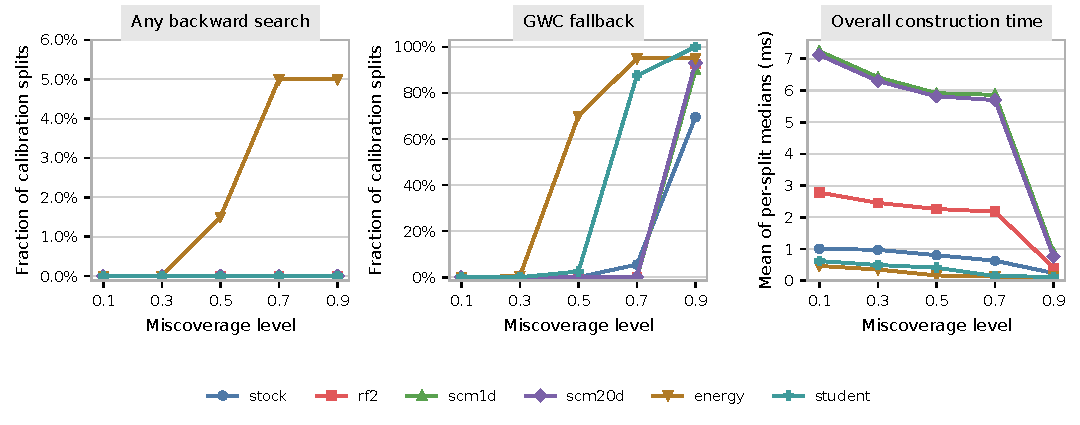
\includegraphics[width=0.98\textwidth]{figures/fig_app_real_search_alpha.pdf}
  \caption{Computational stress sweep on the cached real-data calibration
  residuals. Each point summarizes 200 splits. The first two panels show
  the fractions of splits using any backward search or the global fallback;
  their vertical ranges differ. The final panel reports construction time.
  Additional miscoverage levels use the median of three uninstrumented
  calls per split; the main $\alpha=0.1$ results use seven. All timing
  summaries average these per-split medians.}
  \label{fig:app-real-search-alpha}
\end{figure}

Branch frequencies are measured from the executed algorithm: equality
between TSCP and TSCP-GWC output is not used as a proxy for fallback.
Conditional timings exclude diagnostic logging. These measurements
characterize computation on the evaluated residual samples, not worst-case
search complexity.

\FloatBarrier
\subsection{Monte Carlo Uncertainty}
\label{app:coverage-uncertainty}

We quantify uncertainty for 58 TSCP settings comprising the
independent-observation synthetic studies and the real-data benchmark in
Table~\ref{tab:real-data}. This calculation excludes the fixed-pool studies
and the separate real-data coordinate-analysis batch. The corresponding
nominal target lies within one
across-repetition standard deviation of every reported mean. Only four
synthetic means are below their targets: partial heteroskedasticity at
$n=500$ gives $0.8996\,(0.0164)$; capped-score CQR at $n=50$ gives
$0.8991\,(0.0457)$; $5\%$ contamination gives $0.8995\,(0.0297)$; and
Student $t_{1.5}$ noise at $n=500$ gives $0.8976\,(0.0173)$. Parentheses in
this paragraph contain one standard deviation across repetitions.

For the independent-observation synthetic experiments, training, test, and calibration
observations are independently redrawn, so the repetitions are independent
conditional on the fixed regression coefficients. This interpretation does
not turn repeated splits of a fixed real dataset into fresh population draws. Dividing
the preceding standard deviations by the square root of the number of
repetitions therefore gives a Monte Carlo standard error. The resulting
normal-approximation $95\%$ intervals are, respectively,
$[0.89734,0.90189]$, $[0.88271,0.91541]$, $[0.89536,0.90360]$, and
$[0.89522,0.90003]$; each contains the target $0.9$. Thus, the small displayed
shortfalls are consistent with finite Monte Carlo averaging and do not reveal
a systematic coverage defect in these experiments. Supplementary data
provide the trial-level measurements and pointwise uncertainty summaries.
These normal approximations are not simultaneous confidence intervals or
proofs of coverage. Uncertainty for the real-data coordinate-analysis batch
is reported separately in Appendix~\ref{app:real-coordinate-audit}.

\FloatBarrier
\endgroup
